\documentclass[10pt,draftclsnofoot,onecolumn]{IEEEtran}
\usepackage[margin=0.75in]{geometry}
\usepackage{listings}
\usepackage{underscore}
\usepackage[breaklinks]{hyperref}
\usepackage{url}
\usepackage{breakurl}
\usepackage{graphicx}
\usepackage{atbegshi}% http://ctan.org/pkg/atbegshi
\usepackage{color}

\renewcommand{\refname}{References}
\definecolor{lightgray}{rgb}{.9,.9,.9}
\definecolor{darkgray}{rgb}{.4,.4,.4}
\definecolor{purple}{rgb}{0.65, 0.12, 0.82}

\lstdefinelanguage{JavaScript}{
  keywords={typeof, new, true, false, catch, function, return, null, catch, switch, var, if, in, while, do, else, case, break},
  keywordstyle=\color{blue}\bfseries,
  ndkeywords={class, export, boolean, throw, implements, import, this},
  ndkeywordstyle=\color{darkgray}\bfseries,
  identifierstyle=\color{black},
  sensitive=false,
  comment=[l]{//},
  morecomment=[s]{/*}{*/},
  commentstyle=\color{purple}\ttfamily,
  stringstyle=\color{red}\ttfamily,
  morestring=[b]',
  morestring=[b]"
}

\lstset{
   language=JavaScript,
   backgroundcolor=\color{lightgray},
   extendedchars=true,
   basicstyle=\footnotesize\ttfamily,
   showstringspaces=false,
   showspaces=false,
   numbers=left,
   numberstyle=\footnotesize,
   numbersep=9pt,
   tabsize=2,
   breaklines=true,
   showtabs=false,
   captionpos=b
}

\hypersetup{
    bookmarks=false, % show bookmarks bar?
    pdftitle={Spring Term Report Final Stage}, % title
    pdfauthor={Malcom Diller, Evan Steele, Sean Rettig}, % author
    pdfsubject={Raspberry Pi Outdoor Lighting}, % subject of the document
    pdfkeywords={TeX, LaTeX, graphics, images}, % list of keywords
    colorlinks=true, % false: boxed links; true: colored links
    linkcolor=blue, % color of internal links
    citecolor=black, % color of links to bibliography
    filecolor=black, % color of file links
    urlcolor=blue, % color of external links
  %linktoc=page % only page is linked
}
\title{Not exactly the Internet of Things for Outdoor Lighting\\ Spring Term Report\\ Final Stage}
\author{Oregon State University CS Senior Capstone Group 22\\Malcolm Diller, Sean Rettig, Evan Steele\\Client: Victor Hsu}

\begin{document}
\maketitle
\begin{abstract}
The goal of this project is to create a home lighting automation system from
open source software and inexpensive commodity hardware that allows lights to
be controlled automatically and remotely while also being easy to set up and
use. The system consists of a wireless network of tiny ``client'' computers that
each control up to 4 sets of lights and are controlled by a central ``server''
computer, which automatically sends out commands to the clients when it's
time to turn on or off.  The central node runs a control program that can
be easily accessed via a touch screen, a web browser, or a mobile device, where
the user can locally or remotely control each light individually. The control
interface allows users to easily set ``rules'' for what their lights do and
when, depending on the time of day, the sun/moon position, and potentially even
triggers such as weather conditions or calendar dates.\\

\end{abstract}
\pagebreak
\tableofcontents
\newpage
\section{Introduction}
Since September 2015, we have been developing the final deliverable through several
iterations. The core system was completed for the Winter progress report in the beta
stage, in which all functionality was present. The Spring term was used to polish the
end result and work on various bugs discovered through extensive testing. Our \href{https://github.com/rettigs/cs-senior-capstone}{Github repository} served as our issue tracker, and as the host for our codebase.
Our project has fulfilled the goals that we set out to accomplish, namely having a scheduler for running complex light queries and having an interface for manual control.
The entire system was built on our agreed-upon Python platform of Flask for the web server, where the scripts handled everything from the user interface to sending the TCP commands to the ESP8266 devices.
The final result was prepared using the Yocto build system for deployment on a Raspberry Pi, which automatically fetches the latest build of the application and generates an image with all dependencies satisfied.
The project was extensively tested and debugged before our final presentation.
\section{Status}
For the final release, all core components were completed and debugged,
leaving many quality-of-life changes for the Spring term. Our medium-priority issues were resolved for the final
deliverable. Our full issue list can be
found at \href{https://github.com/rettigs/cs-senior-capstone/issues}{Github}.

\begin{itemize}
    \item Allow option to simulate time running faster\\
	  - For testing purposes, we wanted to have a system where
            we could pass a flag to the startup script and run an entire
            day in a usable time frame.
    \item Better default names for lights\\
          - Early iterations had the light name start as \textit{Light@\textless mac\_address \textgreater},
            which was confusing to read. Better names enhance the user experience.
    \item No login functionality\\
          - A login system was built into the application, however as development
            continued it was decided that it was unnecessary, given that we already
            authenticate to connect to the Pi as an access point.
    \item Jumbled display on mobile devices\\
          - Some of our web design choices were not performing well on mobile
            devices when the light names were long. More nesting in div elements
            fixed this problem.
    \item Server crash on invalid query\\
          - Early iterations of the query thread would cause an exception that would
            end the query runner too soon. Now we handle that exception and just skip
            bad queries.
\end{itemize}
Additionally, we worked on a couple major new features for the project
\begin{itemize}
   \item Reset Button
         - For testing purposes and for the demo, we want a way to show the database
           construction and device addition processes without having to manually
           delete the existing database repeatedly. The reset button clears the
           data and lets us start from scratch.\\ \\
           \includegraphics[width=0.75\textwidth]{reset-button.png}
   \item Poller
         - If multiple screens are open to the light switch page, how do we make sure users don't overwrite each other?
           Using a Javascript poller (using \textit{setInterval}), we now have the main screen update frequently with
           light changes and the configuration of groups and names.
\end{itemize}

Additionally, our final presentation incorporated a little model of a house to demonstrate
a use case for the device. An early prototype was created out of spare PCB and cardboard, with
messy wiring.\\ \\
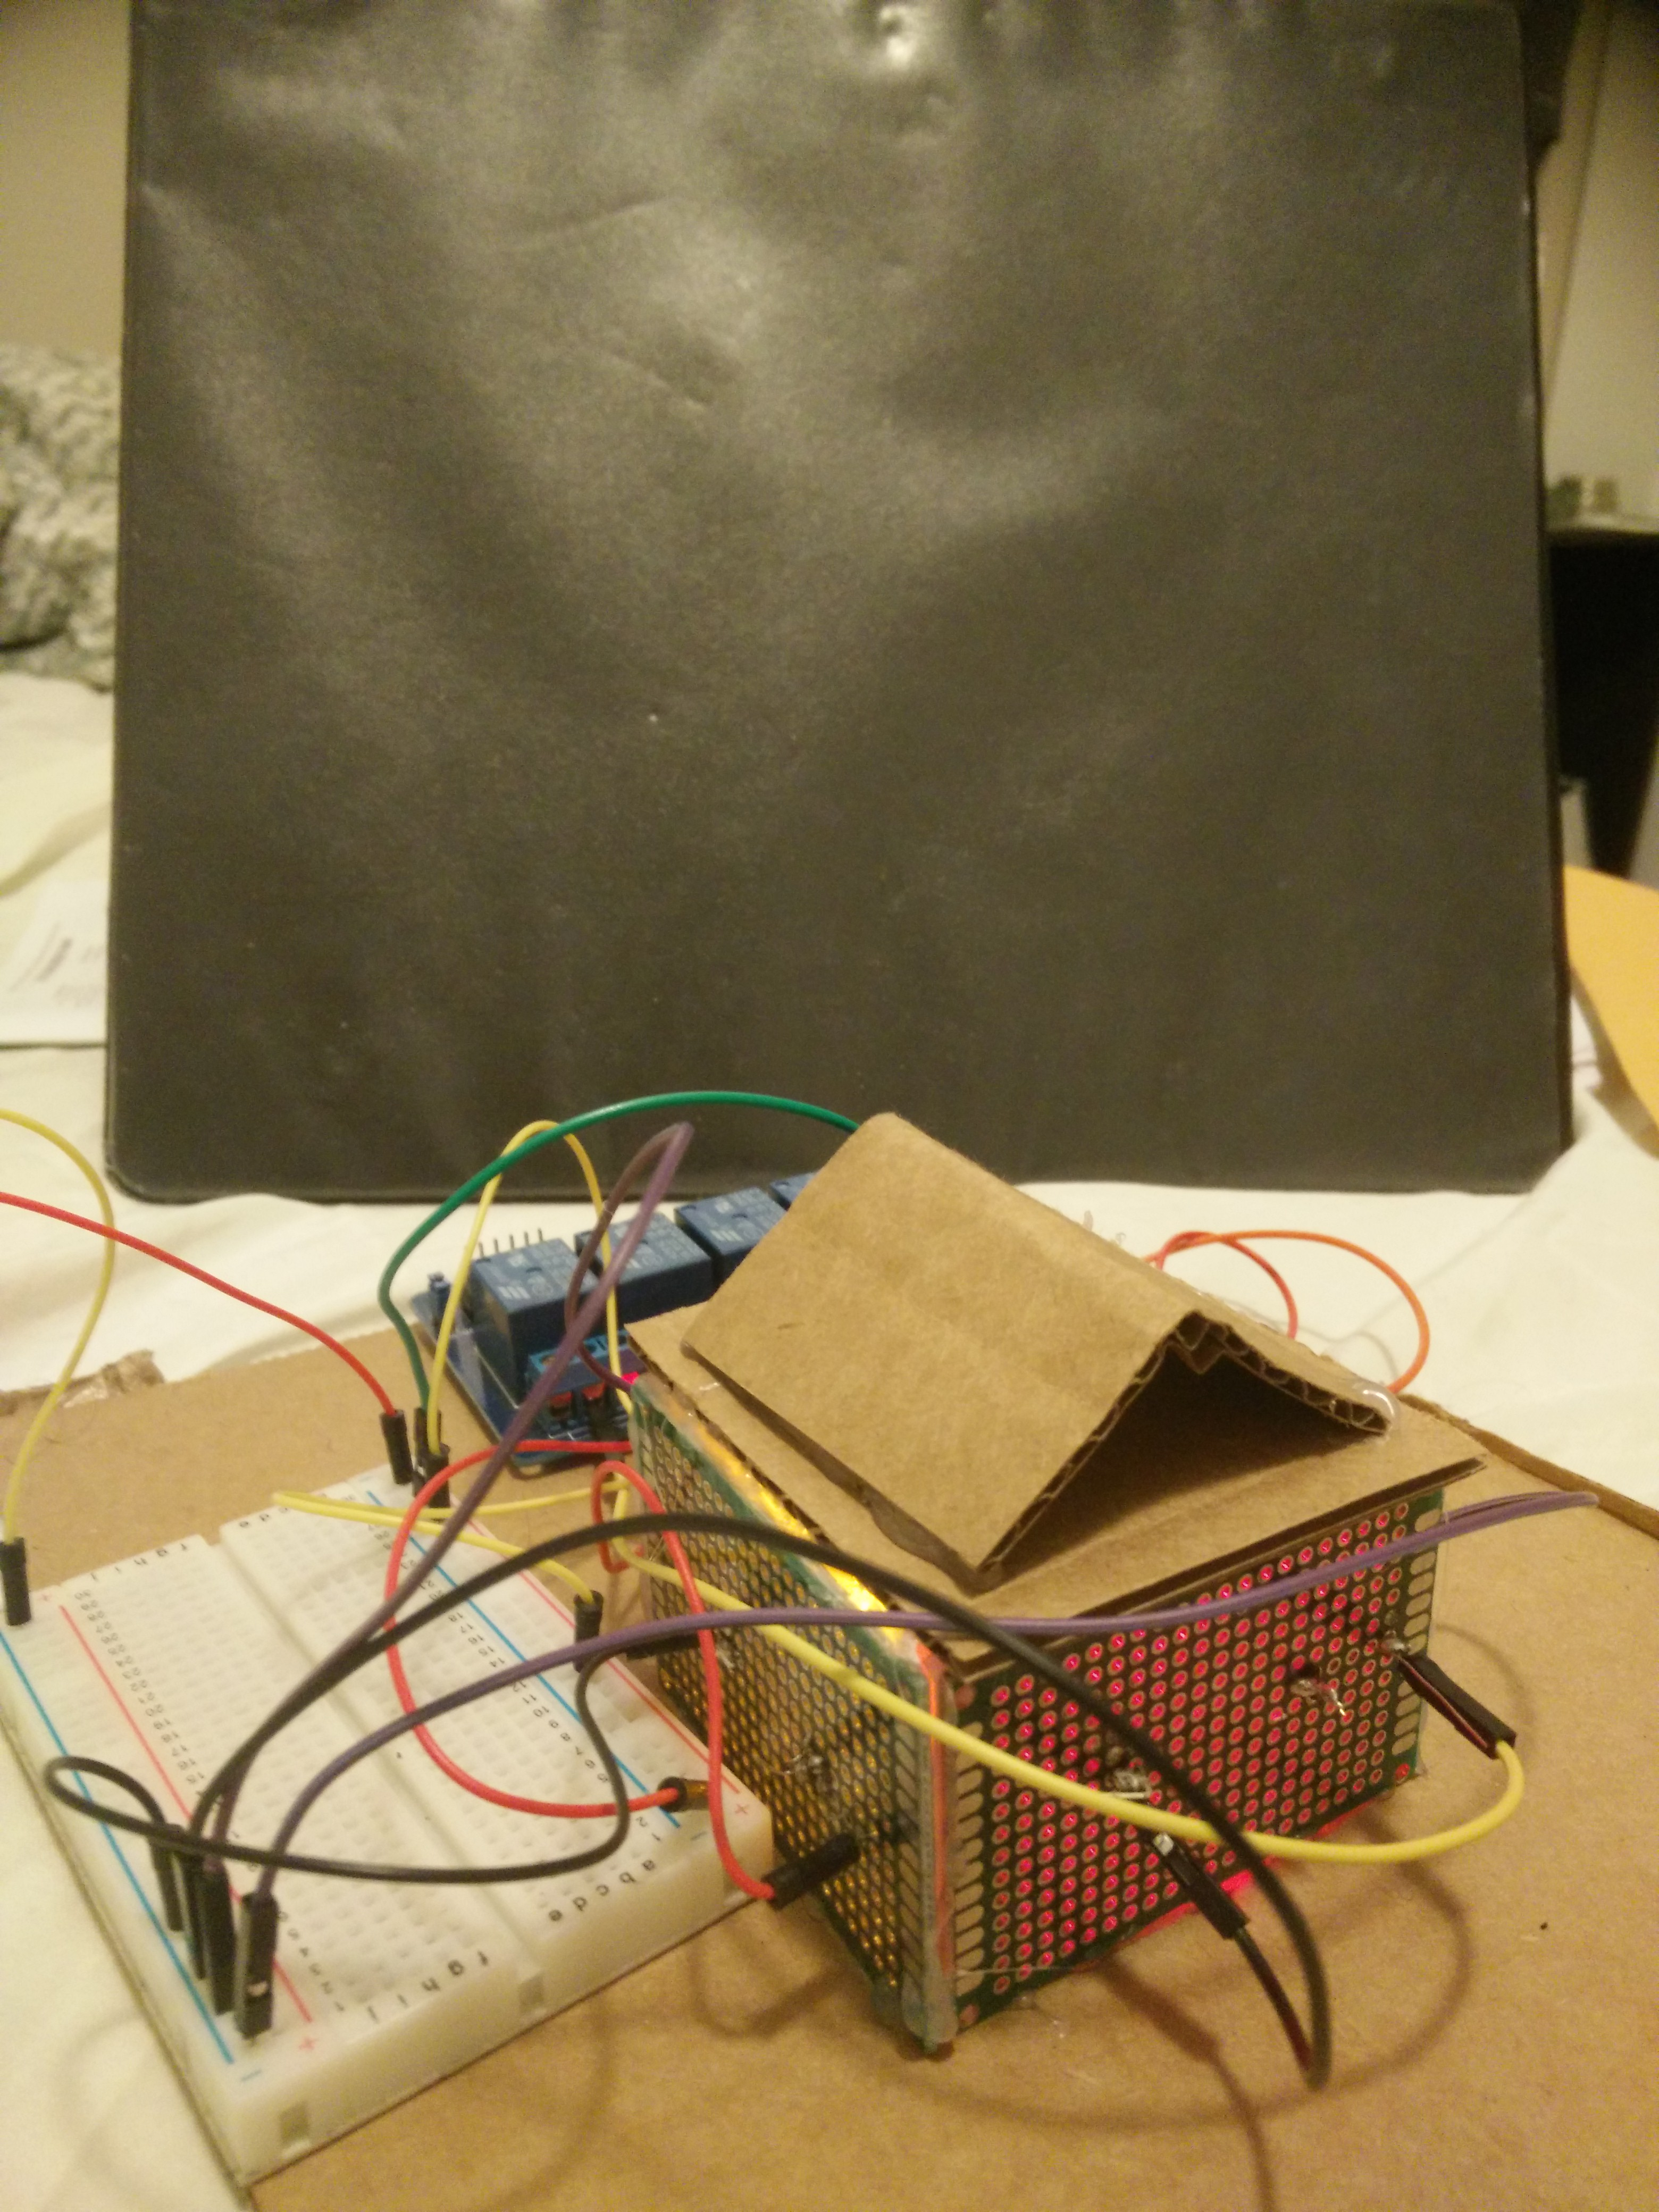
\includegraphics[width=0.75\textwidth,height=7cm]{prototype.png}

\section{Work To Do}
\subsection{Future for Open Source}
Most of our remaining work revolves around small fixes and improvements noted in the
issues list, but the bulk of the work is preparing the project for the open-source community.
The wiki on Github needs to be update to include helpful documentation and some code blocks
require more comments to make the intent of each action more clear. This will ensure that future
contributors can make meaningful progress with the project and deploy it successfully.

Our core goals for the project have been completed on schedule, so there isn't more that absolutely
needs to be accomplished for the final product to be usable. Our expo presentation was created to provide
a compact, physical demonstration and was completed and tested.\\ \\
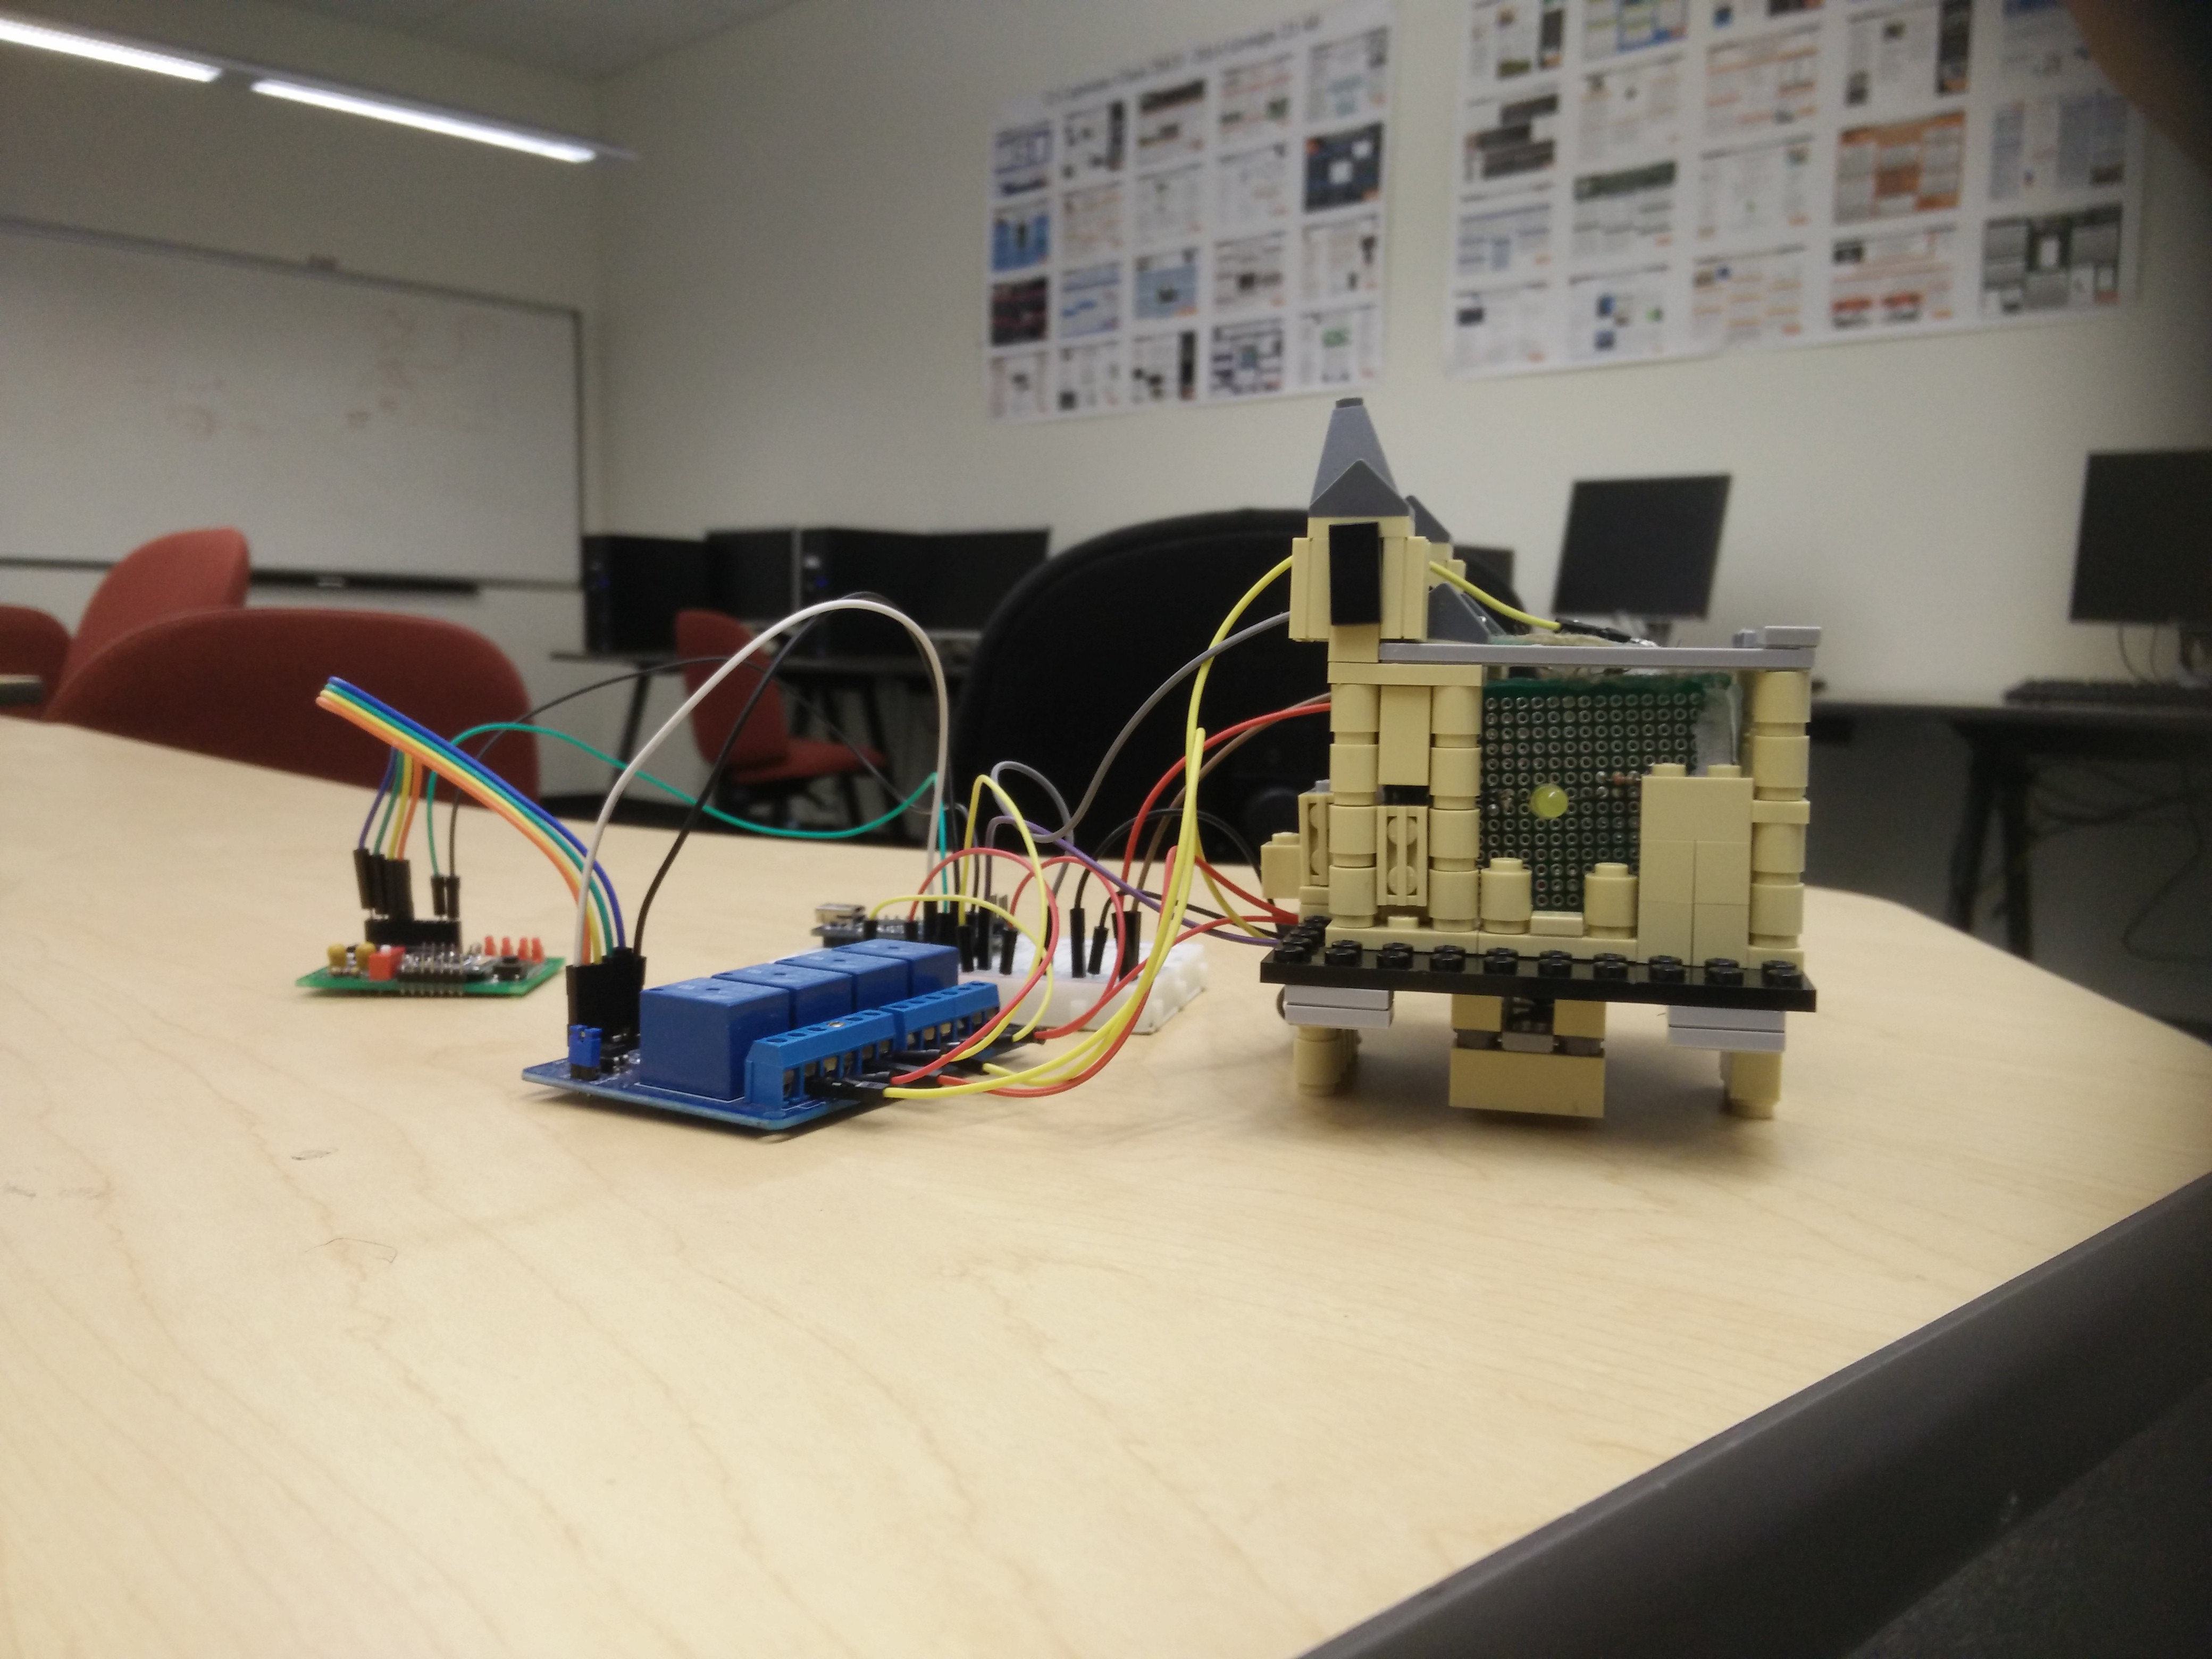
\includegraphics[width=0.75\textwidth]{final-side.png}

\subsection{Low priority issues}
The Github issue list is still populated with low-priority problems that 
mainly focus around usability. The requirements for Expo forced us to look toward
preparing a demo and squashing the bugs that made up the medium and high priority 
issues, but ideally these should all be completed as well. It's unlikely that all of 
these issues will be completed before Expo, but the additional documentation we will
prepare will help the FOSS community take hold of these issues, should interest in the
project develop over time.

\section{Problems}
\subsection{Time Calculation}
A major problem we encountered was on the scheduler for executing queries. We had a major conflict when the times for lights turning on and off was for different days, but where the times were not perfectly aligned for one day. For example, if a light is to turn on at 8pm and off at 6am, the query generated is:\\
\textit{(time \textgreater= qtime('20:00') and time \textless= qtime('06:00'))}\\
But this is never true. A possible solution is adding 24 hours to the off time if the off time takes place before the on time. Actually, this might not work as expected when combined with day-of-week rules. For example, if you want your lights to turn on at 8pm and off at 6am, does that mean:

 \begin{itemize}
 \item They turn on Saturday night and turn off on Sunday morning?
 \item They turn on Friday night and turn off Saturday morning?
 \item They stay on from 00:00-06:00 and 20:00-23:59 on Saturday?
 \end{itemize}

 Since each query can be derived from the original command set, we've hit some major confusion. However, there's not currently any way to modify the times in the query. 
The best solution we got was to add another optional argument to the qtime constructor to indicate that the time should actually be the next day, then on the web interface, setting it on the off time if it's earlier than the on time.

 However, if times are mixed with sunset/sunrise keywords, then we don't actually know which one is earlier until the rule is evaluated, so this needs to be something we calculate at evaluation time. The easiest way to do that is through the qtime object. 
Then we realized that  we can merge both the on and off times into one qtime object that does the calculation automatically.\\
For example, a rule like this:\\
\textit{(time \textgreater= qtime('20:00') and time \textless= qtime('06:00')) and (dow == 5 or dow == 6)}\\
Would be changed to this:\\
\textit{(time \textgreater= qtime('20:00') and (dow == 5 or dow == 6)) or (time \textless= qtime('06:00') and (dow == 6 or dow == 0))}\\
This investigation formed the largest issue we had this term, both in terms of difficulty and focus.
\subsection{Light Switches}
subsection{Behavior of On/Off Switches}

Before starting to implement the rules, we had not put much thought into what
the behavior should be for the On/Off switches of the lights and groups. After
we began to implement more of the project, we realized that there are a few
ways that the behavior could be implemented:

\begin{enumerate}
  \item Toggling the switch would change the state of the light until the user
      chose to resume automated control.
  \item Toggling the switch would change the state of the light for a preset
      amount of time before resuming automated control.
  \item Toggling the switch would change the state of the light until the next
      time that the rules determined the light should change, upon which
      automated control would resume.
\end{enumerate}

For the automation system, we simply don't run the automated query if it involves a 
light that was recently changed manually, until a rule comes up that tells the light
to change again. This allows us to keep the user override in place while also working to
keep the query schedule consistent. When it comes to reflecting the group changes,
we eventually decided on a hybrid system that also involved us redefining how the 
user sees the group lights. If we're going to have the groups behave in a way that was almost
always using the midpoint setting on the Bootstrap switches, we decided that it would be simpler
to just change them to static buttons, not reflecting the status of the entire group. This worked
in conjunction with our decision for the state.\\ \\
\includegraphics[width=0.75\textwidth]{buttons.png}
\subsection{Wireless and Power}

We had an issue early on with how we planned to connect to the ESP8266 modules
using our Raspberry Pi. Our proof-of-concept had the client connecting to the
wireless module itself to make changes, but we wanted remote management to work
from the Pi and have it be reachable from the Internet. We began looking into
ways to perform local routing so that the device could play with the end user's
home network, but ran into more snags trying to configure multiple wireless
network devices on the same Pi. We contacted our client, who suggested that we
not worry about external connectivity for the project. His expectations were
that users would directly connect to the Pi to make configuration changes. The
project title was "not \textit{exactly} the Internet-of-Things", after all.\\

As the project continued, we noticed that it was becoming harder and harder to 
get the ESP8266 devices and the relay on at the same time. When we wired up the 
relay and the module at the same time, the ESP device would just stop broadcasting 
after a few seconds. After spending hours trying to debug the ESP hardware over
FTDI, we found that when they were both connected to the same 5v source, the 
relay itself was eating up most of the power, starving the ESP module. When each device
was moved to individual 5v power supplies (one from a wall outlet and one from an
Arduino Micro over USB), the devices worked well and had enough power for each.
This does mean that the power requirements on the end-user will be stretched for an
actual home implementation, including another source for the Pi, but they
only need 5v supplies, so the drain should not be too taxing.
\subsection{User Interface/Website}

Much of the functionality that we needed for Beta was completed at the Alpha stage.
The database has been created and the main page is currently able to persist
user-submitted data, such as the names of groups and lights.  The advanced page
now triggers server communication utilizing newly created
user-submitted data, using the same core functionality as the front page.

The user interface saw some slight design changes, such as changing the CSS
to make it more friendly for mobile devices by shrinking some elements on the
page. Additionally, the web application has been set to auto-deploy on the Pi
with sufficient error handling when powered on, and it sets the display on the
TFT LCD to properly show the application.

Additional testing with the TFT LCD showed that it would not be
able to handle the full Bootstrap range of features, since the web
browser on the Pi is simply less capable than a deployment of Chrome or
Firefox. Although we anticipated more of an issue, there was no major slowdown
on the Pi itself and the buttons were still present. Scrolling is a bit
difficult, requiring the user to hold onto the device with two hands, 
but that represents the worst issues with the transition to the 3.5 inch screen. \\ \\
\includegraphics[width=0.75\textwidth]{screen.png}

\section{Code}
Not much brand-new code was added to the project this term, but the Javascript poller is completely new. It uses the \textit{setInterval} function like so:\\
\begin{lstlisting}
setInterval(function(){
   var state;
   data = {
      data: "state"
   };
   $.ajax({
      url: "/poll",
      global: false,
      type: "POST",
      cache: false,
      data: data,
      success: function(response){
         for (var key in response) {
            if (response.hasOwnProperty(key)) {
               switch_button = $("li[lid='" + key + "']").find('input');
               if (response[key] == '0'){
                  state = false;
               }else if (response[key] == '1'){
                  state = true;
               }
               console.log(state);
               if (((switch_button).is(':focus'))!=true){
                  switch_button.bootstrapSwitch('state',state);
               }
               state = null;
            }
         }
      }});
},3000);
\end{lstlisting}
This new function is one of the few new site paths we created this term. It needs to constantly
get updates from the database to make sure that the lights on all screens represent the current
state. This poller is exclusively for the switch statuses, but additional pollers are under
development for fetching group statues and names. Mutliple pollers will live in this file,
but we'll still only have one path in the \textit{start.py} server file. We'll just have 
each poller update the data field to identify itself. This particular poller ran every 3 seconds, 
which would be the fastest poller we would want to run.
\section{Concluding Analysis}
Our work this term was more focused around polish and bug fixes than adding any major
new features. Putting together the Expo demo model this term helped expose some 
design issues with the query system and introduced the need for a poller. Compared to
previous terms of work, this was perhaps our lightest, but still intensive as we prepare
to show the core functionality off at Expo. As we presented the build to our client, Victor
earlier this term, he confirmed that the project was moving in the direction he anticipated
and that it was in a presentable state. Based on that assessment and our own goals, 
we are confident in our Expo-ready project.\\ \\ 
\includegraphics[width=0.75\textwidth]{expo.png}
 \newpage
 \Urlmuskip=0mu plus 1mu\relax
 \bibliography{design}{}
 \bibliographystyle{IEEEtran}

 \end{document}
